\documentclass{article}
\usepackage{amsmath, graphicx, amsfonts, caption, subfig, keyval}
\usepackage[numbers]{natbib}
\usepackage{xcolor}
\usepackage{hyperref}
\usepackage[boxruled,procnumbered, linesnumbered]{algorithm2e}
\usepackage[margin=1in]{geometry}
\usepackage{setspace}
\onehalfspacing
\usepackage{csquotes}

\captionsetup{justification=centering}
\newcommand{\R}{\mathbb{R}}
\newcommand{\Rr}{\mathcal{R}}
\newcommand{\D}{\mathcal{D}}
\newcommand{\C}{\mathcal{C}}
\newcommand{\X}{\mathcal{X}}
\DeclareMathOperator*{\argmin}{\arg\!\min}

\doublespacing
\makeatletter
\newcommand*{\toccontents}{\@starttoc{toc}}
\makeatother


\begin{document}
\title{\Huge AM221 Final Project \\ \Large Dictionary Selection Under a Supermodular Assumption}
%\author{ Killian \& }
\singlespacing
\author{
  Taylor Killian\\
           \small Institute for Applied Computational Science\\
	\small 52 Oxford Street\\
	\small Cambridge, MA\\
  \texttt{taylorkillian@g.harvard.edu }
  \and
  Leonhard Spiegelberg\\
         \small Institute for Applied Computational Science\\
	\small 52 Oxford Street\\
	\small Cambridge, MA\\
 \texttt{spiegelberg@g.harvard.edu}
}
\maketitle
\doublespacing
\begin{abstract}
We attempt to develop a method by which to solve dictionary selection under a supermodular assumption. This method is motivated primarily by the work of \citeauthor{Singer16TwoStage}~(\citeyear{Singer16TwoStage}) ~\cite{Singer16TwoStage} where a two-stage submodular maximization generalization was developed. The development of a two-stage supermodular minimization algorithm to address Sparse Dictionary Selection utilizes approximation results derived by Boutsidis et al. (2015)~\cite{weaklyalpha} for supermodular optimization. We show that Sparse Dictionary Selection is functionally equivalent to Sparse Multi Linear Regression which allows us to leverage~\cite{weaklyalpha}. We analyze and experiment with an implementation of our two-stage optimization routine and compare it to current methods. With this project we have laid the ground for further exploration into the formalization of the two-stage method that we propose here.
\end{abstract}

\vfill
\singlespacing
\begin{center}
\bfseries\contentsname
\end{center}
\toccontents
\clearpage

\doublespacing
%%%%%%%%%%%%%%%%%%%%%%%%%%%%%%%%%%%%%%%%%%%%%%%%%%%%
%%-------------------------------                              Introduction                               -------------------------------%%
%%%%%%%%%%%%%%%%%%%%%%%%%%%%%%%%%%%%%%%%%%%%%%%%%%%%
\section{Introduction}\label{sec:intro}

Dictionary selection and sparse regression are variants of representation learning. The goal of these kinds of problems is to determine a sparse representation of input data $X$ in the form of a linear combination of basis elements as well as the basis elements themselves. That is, one essentially factors the input, or design matrix, into a sparse catalog $\mathcal{R}$ and a dictionary of basis elements $\mathcal{D}$, both of which need to be inferred from the data.\\

%%%%%%%%%%%%%%%%
%%    Problem Definition     %%
%%%%%%%%%%%%%%%%
\subsection{Problem Definition}\label{sec:problem}
\noindent Dictionary learning, in its general form, can be seen as an optimization problem
\[
\min_{\D, \Rr, \theta, \lambda} f(\D, \Rr, X) + g(\D, \theta) + h(\Rr, \lambda)
\]
where $f$ describes the objective function used to measure goodness of approximation of $X$ through $\D, \Rr$, $g$ describing suitable constraints on the dictionary, $h$ on the representation respectively.\\

\noindent With an input dataset $X=[x_1, \dots, x_k],  x_i \in \R^d,  X \in \R^{d\times k}$ we wish to find a dictionary\\
$\D \in \R^{d\times n}, \   \D~=~[d_1, \dots, d_n]$ and a representation $\Rr \in\R^{n\times k}, \ \Rr = [r_1,\dots,r_k], \ r_i\in\R^n $  such that both $\|X-\D\Rr\|_F^2$ is minimized (with $\| . \|_F$ describing the Frobenius norm defined by $\|A\|_F := \sqrt{\sum_i\sum_j |A_{ij}|^2}$) and the representations $r_i$ are ``sparse enough". To limit the dictionary becoming infinitely large (or small) we introduce a constraint on the dictionary's columns. For this any sufficient norm can be used. An often used norm is the $l_2$-norm. 
Thus, for the dictionary learning problem we introduce the problem with constraints
\begin{align*}
         &\min_{\D, \Rr} \ \|X  -\D \Rr\|_F^2   \quad   \\
         \text{s.t.}  \quad  &\|d_j\|_2 \leq 1, \quad \forall j=1, ...,n  \quad \\
          \quad  &\|r_i\|_0 \leq t,  \quad \forall i=1, ...,k  \quad 
\end{align*}

\noindent Here the constraints express the expectation that both $\D$ is controllably determined and that $\Rr$ is adequately sparse. The difficulty in solving this problem comes from the mathematical challenge the $\| . \|_0$ norm yields. This norm is defined as:\\ 

\qquad\qquad\qquad\qquad Let $x \in \R^d$
\[
\ell_0(x) := \big|\{x_i : x_i \not= 0\}\big|
\]That is, there are at most $t$ non-zero columns in $\Rr$. By using Lagrange multipliers this can be brought to the general form above
\[
\min_{\D, \Rr, \theta, \lambda} \|X  -\D\Rr\|_F^2 + \sum_{j=1}^m \theta_j (\| d_j\|_2 - 1)+ \sum_{i=1}^k \lambda_i (\| r_i \|_0 - t)
\]
I.e. the functions are
\[
\begin{split}
f(\D, \Rr, X) &:= \| X -\D \Rr \|_F^2 \\
g(\D, \theta) &:= \sum_{j=1}^n \theta_j (\| d_j\|_2 - 1) \\
h(\Rr, \lambda) &:= \sum_{i=1}^k \lambda_i (\| r_i \|_0 - t)
\end{split}
\]
%\autoref{fig:l012plot}.
%\begin{figure}
%\centering
%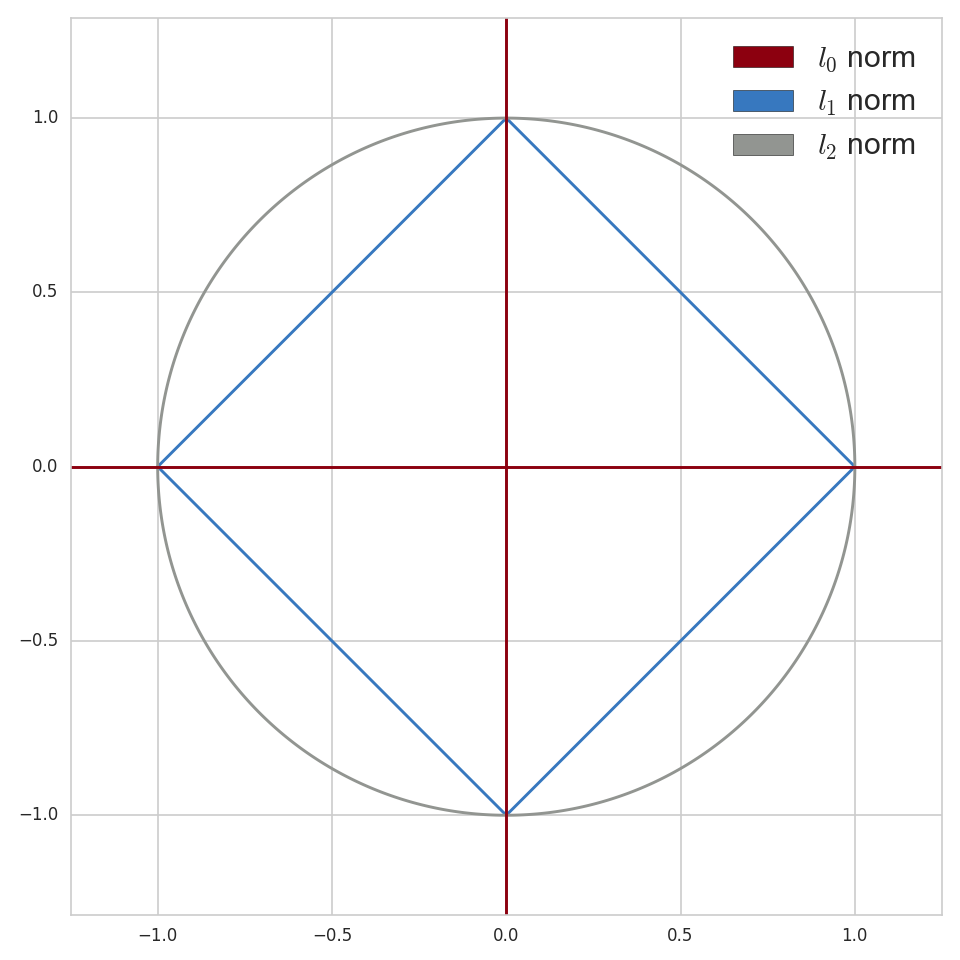
\includegraphics[scale=0.3]{img/l012_norms.png}
%\caption{contour plot of the $l_0, l_1, l_2$ norm at levelset $L_1(f) := \lbrace x \in \R^2 : f(x) = 1 \rbrace $. Note that for any space $\R^d$, the image of the $l_0$ consists of $d+1$ values ($\lbrace 0, ..., d \rbrace $).}
%\label{fig:l012plot}
%\end{figure}


%%%%%%%%%%%%%%
%%     Prior Work          %%
%%%%%%%%%%%%%%
\subsection{Related Work}\label{sec:prior-work}

In order to tackle the problem whose complexity mainly arises from the $\| .\|_0$ norm, one approach is to relax the norm to a more feasible one (i.e. LASSO, LARS for convex-relaxation or log penalty for non-convex relaxation). However, this might lead to over-penalization~\cite{nonconvexrelax}. Another ansatz is to utilize a greedy approach which constantly adds or removes variables based on some measure~\cite{submod_spectral}.  Another method attempts to adjust the dictionary and sparse representation in an online fashion~\cite{mairal09}. This can be stated as a maximization problem of a submodular function. A submodular function thereby can be viewed as a discrete analog to a convex function in the continuous case~\cite{submod_sparsecoding} which encodes the principle of ``diminishing returns". These submodular approximations to Sparse Dictionary Selection have become nearly ubiquitous in the literature with slight algorithmic variations that approach the theoretical bounds, $(1 - 1/e)$, set in~\cite{Krause05near-optimalnonmyopic}.
\\

\noindent Applications of Sparse Dictionary Learning---in particular the utilization of submodular approximations---are broad and varied; with uses found in classical Machine Learning (i.e. Sparse Linear Regression), Computer Vision (Image reconstruction, inpainting, denoising), Signal Processing~\cite{submod_sparsecoding}~\cite{nonconvexrelax}, Social Network Analysis, Statistics~\cite{rIBP}, and Economics~\cite{utilityWelfare} among many others. 
\\

\noindent There has been little work in Sparse Regression and Dictionary Learning that utilize the functional inverse of submodular approximations, known as supermodular functions. Supermodularity can facilitate the potential formulation of a dual to the native Dictionary Learning problem. Recently there has been some attempts at developing foundations for extending the suite of algorithms used in submodular maximization to supermodular formulations. In order to accomplish this, several caveats have been made on the functional representations themselves~\cite{weaklyalpha}. We leverage the gains made in submodular optimization and use recent results in approximating supermodular functions in constructing a two-stage supermodular minimization extension of the continuous greedy algorithm used in the submodular case~\cite{Singer16TwoStage}.

%%%%%%%%%%%%%%%
%%     Supermodularity     %%
%%%%%%%%%%%%%%%
\subsection{Supermodular Assumption}\label{sec:supermod}

\noindent Typical optimization problems that use submodular or supermodular set functions are generally of the form:\\
\noindent Given a set of objects $V=\{v_1,\ldots,v_n\}$ and a function $f:2^V\to \R$ that returns a real value for any subset, find an optimal subset $S \subseteq V$ that optimizes $f$.
\\
\\
Since we are interested in finding a dictionary $\D$ and coding (or representation) $\Rr$, our objective function becomes the error that arises when reconstructing $X$ with $\D \text{ and } \Rr$ and the set $V$ is represented by the columns of $X$ we choose to determine $\D$, and later use to solve for $\Rr$, with. In solving the minimization we iteratively select a subset $S\subseteq X$ according to ${\argmin}_{S\subseteq X} f(S)$,  subject to some constraints on the size of $S$. As was expressed in~\ref{sec:problem}, we can see that our general formulation of Dictionary Selection:  
$$\min_{\D, \Rr, \theta, \lambda} \|X  -\D\Rr\|_F^2 + \sum_{j=1}^m \theta_j (\| d_j\|_2 - 1)+ \sum_{i=1}^k \lambda_i (\| r_i \|_0 - t)$$
can be expressed in supermodular forms.\\

\noindent The remainder of this paper is focused on the development of a two-stage supermodular minimization algorithm. We build up to this algorithm via discussion and analysis of recent results. We present a framework of our two-stage minimization method for dictionary selection and compare it to other commonly implemented algorithms, e.g. MOD and  ``Online" learning.

%%%%%%%%%%%%%%%%%%%%%%%%%%%%%%%%%%%%%%%%%%%%%%%%%%%%
%%--------------------             Setting up the Analysis/Developing the Algorithm                --------------------%%
%%%%%%%%%%%%%%%%%%%%%%%%%%%%%%%%%%%%%%%%%%%%%%%%%%%%
\section{Analysis and Extension of Recent Results}\label{sec:recentresults}

This section is dedicated to a brief analysis and extension of two recent results that we leverage in the development of a two-stage supermodular minimization algorithm. The first is the development of a generalized two-stage submodular maximization algorithm~\cite{Singer16TwoStage}, that we use as a guide in the development of our own supermodular algorithm. The second is the development of supermodular minimization techniques based on an approximation of the supermodular functions used to express various objectives~\cite{weaklyalpha}. We include a brief discussion of these approximation methods. The primary example that the authors use to demonstrate their approximation method is that of Sparse Multiple Linear Regression (SMLR). We show that SMLR is functionally equivalent to Dictionary Selection and that Dictionary Selection is inherently a two-stage problem. This fact allows us to directly use the results from~\cite{weaklyalpha} as a fundamental part of solving for the sparse representation $\Rr$, shown below in Section~\ref{sec:algorithm}.

\subsection{Weakly-$\alpha$ Supermodularity} \label{weakalpha}

Weakly-$\alpha$-supermodularity is a relaxation of supermodularity. With this relaxation, it can be shown that problems that are $\alpha$-weakly supermodular can be solved using a slightly adapted standard greedy algorithm. However, convergence typically requires more steps than  if the problem was supermodular only.
\\
\\
A non-negative, non-increasing set function $f(S): 2^{[n]} \rightarrow \mathbb{R}^+$ is weakly-$\alpha$-supermodular if there exists $\alpha \geq 1$ such that for any two sets $S, T \subseteq [n]$
\[f(S) - f(S \cup T) \leq \alpha \vert T \setminus S\vert \max_{i \in T \setminus S} f(S) - f(S \cup \lbrace i \rbrace) \]
To understand the definition better, assume we are given two disjoint sets $A, B \subseteq [n]$ with $A \cap B = \emptyset$. Then $\alpha$-weakly-supermodularity means that we can find an element $i \in B$ s.t. 
\[
\frac{f(A) - f(A \cup B)}{\alpha \vert B\vert} \leq f(A) - f(A \cup \lbrace i \rbrace)
\]
In words, we can find an element $i$ that is better (in terms of lowering the objective function) than $\frac{1}{\alpha}$ times the average gain of an element of $B$\footnote{Note that for a supermodular function $\alpha = 1$}.
\\
\\
In order to solve the SMLR problem given a relaxed supermodular formulation
\[\min \lbrace f(S) : \vert S \vert \leq k \rbrace \]
for some $k$, the greedy extension algorithm needs at most 
\[ \left\lceil \alpha k \ln \left(f\left(\frac{S_0}{\epsilon}\right)\right)\right\rceil \]
 steps given a start solution $S_0$ (usually the empty set), a threshold error $\epsilon$ (i.e $f(S_k) \leq (1+\epsilon)f(S^*)$ for the optimal solution $S^*$) and the weakness-parameter $\alpha$ of the function $f$ \cite{weaklyalpha}.
 \\
 \\
As in \cite{weaklyalpha} the authors show that sparse regression can be seen as minimizing a $\alpha$-weakly supermodular function with $\alpha = \| X^+ \|_F$, the extended greedy algorithm presented can be used to solve sparse regression.

\subsection{Dictionary Selection as Two-Stage Supermodular Minimization} \label{supermodTwoStage}

Here we highlight the functional equivalence of Dictionary Selection to SMLR, aided by the fact that both problems are under the umbrella of Representation Learning. The goal of demonstrating the equivalence of SMLR and Dictionary Selection is that we can extend the theoretical guarantees and algorithmic foundations in~\cite{weaklyalpha} in our future work. \\

\noindent SMLR is defined as follows:\\
Given two matrices $X\in\R^{m\times n}$, $Y\in\R^{m\times l}$ and an integer $k$, find a matrix  $W\in\R^{n\times l}$ that minimizes $\|XW-Y\|^2_F$ subject to $W$ having at more $k$ non-zero rows. This problem is usually paired with a common assumption/simplification, where the columns of $X$ are adjusted to have unit norm.
\\

\noindent As outlined in \autoref{sec:problem}, here is a general definition of the Dictionary Selection problem.
\begin{alignat}{5}
         & \argmin_{\D, \Rr} \|X \ -&\D\Rr\|_F^2  + &\lambda \sum_{i=1}^k  \|\ r_i\|_0     \quad   \\
         &\text{s.t.}  \quad  &\|d_j\|_2 \leq 1&, \forall j=1, ...,n  \quad 
\end{alignat}
Thus, given an input dataset $X=[x_1, \dots, x_k], \ x_i\in\R^d, \ X\in\R^{d\times k}$ we wish to find the dictionary $\D\in\R^{d\times n}, \ \D = [d_1, \dots, d_n]$ and a representation $\Rr=[r_1,\dots,r_k], \ r_i\in\R^n, \ \Rr\in\R^{n\times k}$, such that both $\|X-\D\Rr\|_F^2$ is minimized and the representations $r_i$ are "sparse enough" (can be specified column by column as in \cite{rIBP}, or be extended as defined in SMLR).\\
\\
\noindent In SMLR, the data matrix $X$ with the determined, sparse $W$, are used to approximate $Y$ while in Dictionary Selection the matrices $\D,\ \Rr$ are determined to approximate the data $X$. In both problems, sparse representations are used to select a combination of data that closely replicates known data. For all intents and purposes these two problems are functionally equivalent with consideration being made to ensure that the sparsity requirements of Dictionary Selection (where there is a limit on the sparsity of each row/column) port into those of SMLR (where the sparsity requirements are placed on the matrix in full). This isn't of too much concern as this can be handled in the definition of each specific application of the Dictionary Selection problem.\\
\\
Observing that the definition of the dictionary selection problem (Equation 6) requires the minimization over the matrices $\D\text{ and }\Rr$ when taken together, this problem is combinatorially infeasible~\cite{NPHardproof} and non-convex. However, if we separate the problem into a two-stage optimization (where we fix one matrix and solve for the other and then iterate) we can apply well understood convex solution strategies.~\cite{submod_spectral}, \cite{greedy_selection}, \cite{rIBP}, \cite{Singer16TwoStage}. These two stages are: 
\begin{enumerate}
\item Fix $\D$, find a sparse coding between it and $X$.
\item Solve the Dictionary Optimization problem: $\D = X\Rr^{+}$ following which we renormalize $\D$.
\end{enumerate}
Upon iteration we can expect convergence, using guarantees in the continuous greedy algorithm~\cite{greedy_selection}, \cite{submod_spectral}, \cite{submod_sparsecoding} as well as those made in \cite{weaklyalpha}. The commonly known sparse regression can be seen as an instance of sparse multiple linear regression with $Y$ existing only of one column. I.e. $XW-Y$ is a vector. 

%%%%%%%%%%%%%%%%%%%%%%%%%%%%%%%%%%%%%%%%%%%%%%%%%%%%
%%----------------------------                                    Algorithm                                      ---------------------------%%
%%%%%%%%%%%%%%%%%%%%%%%%%%%%%%%%%%%%%%%%%%%%%%%%%%%%
\section{Two-stage Supermodular Minimization Algorithm}\label{sec:algorithm}

Recall the general form of the Dictionary Selection Problem we introduced in \autoref{sec:problem}:

$$\min_{\D, \Rr, \theta, \lambda} \|X  -\D\Rr\|_F^2 + \sum_{j=1}^m \theta_j (\| d_j\|_2 - 1)+ \sum_{i=1}^k \lambda_i (\| r_i \|_0 - t)$$

\noindent We now relax the problem by formulating it into the two stages described above:
\begin{enumerate}
\item solve for fixed $\D, \theta$ the minimization to obtain optimal $\Rr, \lambda$.
\item solve optimization for $\D, \theta$ with obtained values
\item repeat previous steps until done
\end{enumerate}

\noindent In generic terms, this is similar to the method of optimal directions. In the traditional method of optimal directions~\cite{MOD} the subproblem $\min_{\Rr, \lambda} f(\D, \Rr, X) + g(\D, \theta) + h(\R, \lambda)$ is solved by various relaxation methods (i.e. LASSO, Matching Pursuit, etc.), however for our approach we want to embed the problem into a combinatorial optimization framework, which guarantees us bounds on optimality. Using~\cite{weaklyalpha} we reformulate the Dictionary Selection with $\alpha$-weakly supermodular functions. We will now show how to obtain this formulation:
Recall that
\begin{align*}
\min_{\Rr, \lambda}\quad &f(\D, \Rr, X) &+& \qquad\qquad g(\D, \theta) &+& \qquad\qquad h(\Rr, \lambda) \\
= \min_{\Rr, \lambda}\quad &\|X -\D \Rr\|_F^2 &+& \qquad\qquad\sum_{j=1}^n \theta_j (\| d_j\|_2 - 1) &+& \qquad\qquad\sum_{i=1}^k \lambda_i (\| r_i \|_0 - t)
\end{align*}
then let $S \subseteq [n]$ be a set of column indices for the dictionary. From now onwards we will assume that the given, fixed dictionary is normalized, i.e. $\forall d_i: \|d_i \|_2 = 1$. This allows us to remove the term $g(\D, \theta)$. Define now $\D_S$ as the matrix obtained from $\D$ with all columns not indexed by $S$ to be set to zero.
\[
(\D_S)_{ij} := \begin{cases}
0 \quad &j \notin S \\
\D_{ij} \quad &j\in S
\end{cases}
\]

\noindent$\D_S^+$ is the pseudoinverse which can be obtained i.e. via singular value decomposition when $\D_S = U\Sigma V^T$ through $\D_S^+ = V \Sigma^+ U^T$.
Then the problem can be equivalently stated as
\[
\begin{split}
 \min_{\Rr, \lambda} \|X  -\D \Rr\|_F^2 + \sum_{i=1}^k \lambda_i (\| r_i \|_0 - t)\\
 \Longleftrightarrow 
  \min_{S \subseteq [n], |S| \leq t} \|X  -\D_S\D_S^+ X\|_F^2
 \end{split}
\]
\cite{weaklyalpha} have shown that the objective function $f(S) := \|X  -\D_S\D_S^+ X\|_F^2$ of this optimization problem is $\alpha$-weakly supermodular with 
\[ 
\alpha = \max_{\tilde{S} \subseteq [n]}\| \D_{\tilde{S}}^+ \|_F^2
\]

\subsection{Combination and algorithm formulation}
For the two stage formulation we can generally think of the problem as of adapting the idea of the method of optimal directions but instead of projecting the given representation onto the dictionary we strive for an additional minimization problem:
Let $f_1, ..., f_m$ be instances of the SMLR problem with different dictionaries $\D_k$
\[
f_k := \min_{\D_k, \Rr, \lambda} \|X  -\D_k \Rr\|_F^2 + \sum_{i=1}^k \lambda_i (\| r_i \|_0 - t)
\]
 Then the dictionary problem can be seen as
\[
\min_{\D, \theta} q(f_1, ..., f_m) + \sum_{j=1}^n \theta_j (\| d_j\|_2 - 1)
\]
for some combination function $q$. We now ask, which properties such a combination function ideally should satisfy. One desirable property would be $q$ to be modular as this ensures the composition to be $\alpha$-supermodular\footnote{A proof for this should be developed, but is presumably analogous to the one for supermodular/modular functions}.
 \ \\
 One choice for $q$ could be 
 \[q(f_1(\D, \theta), ..., f_m(\D, \theta)) := \sum_{i=1}^m f_i(\D, \theta)\]
ensuring $\alpha$-supermodularity\footnote{due to modularity of the sum function}, another one to minimize the product of the SMLR instances. Reformulating it with a logarithm might give even better results with increased computationally tractability 
 \[
 q(f_1(\D, \theta), ..., f_m(\D, \theta)) = \sum_{i=1}^m \log (f_i(\D, \theta))
 \]
 \\
 The complete formulation as a two stage problem can be written as 
 \[
 \min_{\substack{S : |S| \leq t}} \sum_{j=1}^m \min_{\substack{S \subseteq T:\\ |T| \leq \min \lbrace 2t, n \rbrace}}f_j(T)
 \]
 with $f_j(T) = \|X  -\D_T\D_T^+ X\|_F^2$.
 \subsubsection*{Algorithm proposal}
 In the following we propose a general randomized greedy algorithm to solve the dictionary learning problem.
 
 \begin{centering}
\begin{algorithm}[H]
\SetKwData{Left}{left}
\SetKwData{This}{this}
\SetKwData{Up}{up}
\SetKwFunction{RandomDict}{RandomDictionary}
\SetKwFunction{alphaSup}{$\alpha$-GreedySolver}
\SetKwInOut{Input}{input}\SetKwInOut{Output}{output}

\Input{A data matrix $X \in \R^{d \times k}$}
\Output{A dictionary $\D \in \R^{d \times n}$ and representation $\Rr \in \R^{n \times k}$}

$D_0 \gets$ \RandomDict{$-1$, $1$} \tcp*[f]{assert $\D_0 \not= 0$} \\
normalize s.t. $\| (\D_0)_{*j}\|_2 = 1$\\
$S_0, \Rr_0 \gets $ \alphaSup{$X$, $\D$, $t$}\\
$m \gets 0$\\
 \While{$m < \mathrm{MAXSTEPS}$ }{
 	$\D_{m+1} \gets X_{S_m \setminus \lbrace q\rbrace \cup \lbrace p\rbrace}$\\
	normalize s.t. $\| (\D_{m+1})_{*j}\|_2 = 1$\\
	$S, \Rr \gets $ \alphaSup{$X$, $\D_{m+1}$, $t$} \\
	\If{$\| X - \D_{m+1}\Rr\|_F^2 < \| X - \D_m\Rr_m\|_F^2$} {
		$S_{m+1}, \Rr_{m+1}  \gets S, \Rr$
	}
	$m \gets m + 1$\\
  }
 \caption{General randomized greedy algorithm for Sparse Dictionary Learning}
 \label{algo:randgeneral}
\end{algorithm}
\end{centering}
\ \\

\noindent We start by initializing a non-zero random dictionary (excluding $0$ as trivial solution). To allow for all directions, negative and positive values are permitted. To restrict the dictionary size, normalization along columns is done in lines $2$ and $8$. We use the greedy algorithm as proposed in~\cite{weaklyalpha} in lines $3, 8$ to solve for a given dictionary the SMLR problem by using $t$ steps (yielding $t$ columns for representation). The indices of the columns that best solve the SMLR are returned as set $S$ along a representation $\Rr$. We then iteratively refine the solution.
\\
\\
Therefore one observation is crucial: Given a set of columns $S$ that represents the indices of non-zero columns of $R$, only $|S|$ corresponding columns in $D$ obtained through matrix multiplication will contribute value-wise to the norm. Thus, in order to improve the solution we need to exchange one (or more) columns of the current set $S$ with some other column that might give a better solution. To obtain a new dictionary candidate we construct it by using a similar argument via the data matrix $X$. I.e. choose randomly a column index $q \in S$ that will be removed and add another random column index $p \in \lbrace 1, ..., k \rbrace \setminus S$. This step is performed in line 7, \ref{algo:randgeneral}. We then obtain the dictionary candidate by $l_2$-column normalization and solve the resulting SMLR problem via the $\alpha$-weakly supermodular greedy algorithm. If the new solution is better than the old one, we keep it, else we perform another round of local search.
%%%%%%%%%%%%%%%%%%%%%%%%%%%%%%%%%%%%%%%%%%%%%%%%%%%%
%%----------------------------                                      Results                                      ---------------------------%%
%%%%%%%%%%%%%%%%%%%%%%%%%%%%%%%%%%%%%%%%%%%%%%%%%%%%
\section{Results}\label{sec:results}

In this section we briefly compare the results of how the approximation algorithm detailed in Section~\ref{sec:recentresults} performs on SMLR in comparison with other well established methods. The two methods that we chose to evaluate due to their straight forward implementation were those of Method of Optimal Directions (MOD)~\cite{MOD} given its close relationship and the ``Online" dictionary learning algorithm developed by Mairal et. al~\cite{mairal09}. We also evaluate the performance of our algorithm against a notional bound which is just the naive inversion of the equation $\D_0\Rr = X$ where $\D_0$ is the initial dictionary omitting any constraints posed on columns of $\D_0$. That is, we compare the performance of our algorithm against the bound $\|X-\D_0\Rr_0\|_F^2$ where $\Rr_0 = \D_0^+ X$.

\subsection{Weakly-$\alpha$ Minimization v. MOD, ``Online" Dictionary Learning}

The Method of Optimal Directions is an example of a two-stage iterative method used to calculate the sparse registration and dictionary of basis elements given some input data. What MOD does is that it takes in an initial $\D_0$, solves for $\Rr_0$ via some sparse coding algorithm (we used LARS) and then updates the estimate of $\D$ by evaluating the singular value decomposition of the sparse registration $\Rr_0$. Using the left and right singular vectors along with the reciprocal of the singular values the pseudoinverse solution to $X = \D\Rr$ for $\D$ is approximated. After applying these stages a number of times, the values converge to the optimal choices for $\D$ and $\Rr$.\\

\noindent The online approach suggested by Mairal et. al.~\cite{mairal09} also takes in an initial dictionary $\D_0$ and solves for $\Rr_0$ via some sparse registration algorithm (again, we used LARS). Rather than directly solving for an updated $\D$, the online method creates a rank one update to $\D_0$ using the sparse columns of $\Rr_0$ and the corresponding rows of $X$. This update acts as a form of gradient descent while iteratively minimizing the objective $\|X-\D\Rr\|_F^2$ over a set number of iterations.\\

\noindent We show the results of applying the methods described above in comparison with the weakly-$\alpha$ solution from Section~\ref{sec:recentresults} over 25 steps. We generate a random design matrix $X$ as well as an initial $\D_0$ and then generate the best sparse registration $\Rr$ and dictionary $\D$ according the three algorithms in an attempt to minimize the SMLR objective. The results of this exploration are summarized in Figure~\ref{fig:smlr}.

\begin{figure}[ht!]
\centering
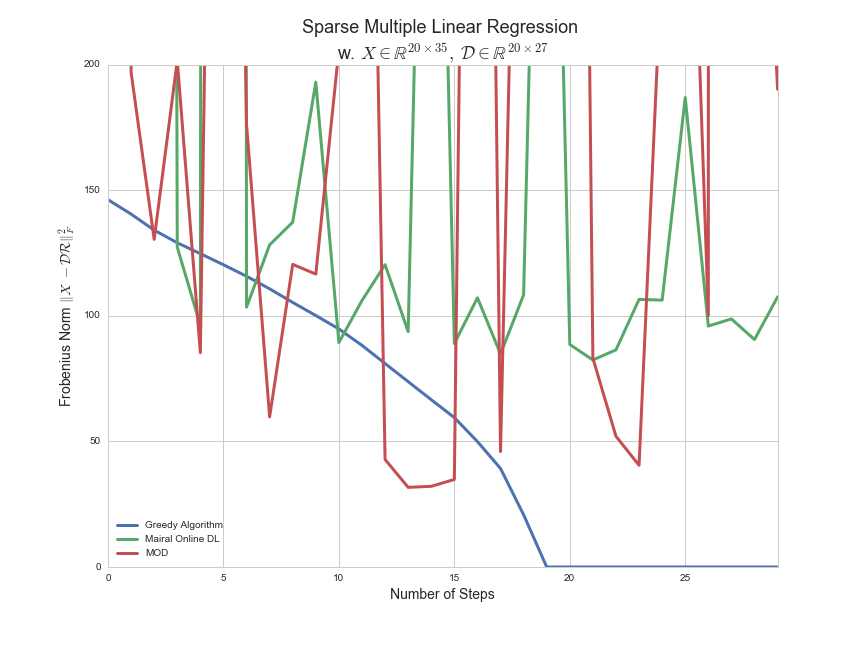
\includegraphics[width=0.65\textwidth]{src/sparse_MLR_greedy_online.png}
\caption{Comparison of three separate algorithms in the solution of SMLR. Note that both MOD and Online Learning are highly unstable.}
\label{fig:smlr}
\end{figure}

\subsection{Performance of Our Algorithm}

As shown in Figure~\ref{fig:ouralg}, our algorithm improves on the naive bound we described above (in some cases). This is a great first step for us as we can see that our proposed method of minimizing the reconstruction error of a given design matrix by a dictionary of learned basis vectors and a sparse registration is working. We are encouraged to continue to refine and develop this method further now that we have it in place. Good things are ahead!

\begin{figure}[ht!]
\centering
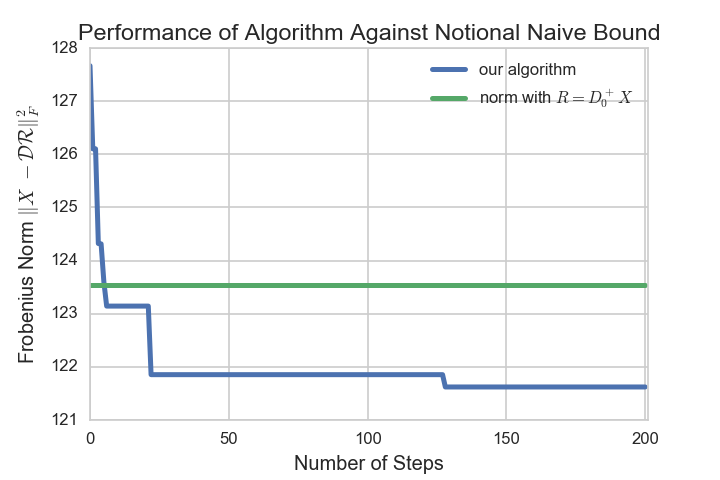
\includegraphics[width=0.65\textwidth]{src/our_alg.png}
\caption{The performance of our proposed algorithm with $t=4$ out of $\binom{27}{4} =17,550$ possible column sets in comparison to a naive bound. }
\label{fig:ouralg}
\end{figure}



%%%%%%%%%%%%%%%%%%%%%%%%%%%%%%%%%%%%%%%%%%%%%%%%%%%%
%%----------------------------              Conclusion/Future Steps/Discussion                ---------------------------%%
%%%%%%%%%%%%%%%%%%%%%%%%%%%%%%%%%%%%%%%%%%%%%%%%%%%%
\section{Conclusion}\label{sec:conclude}
This paper summarizes the development of a two-stage approach to supermodular minimization applied to Dictionary Selection which utilizes recent results from~\cite{weaklyalpha} and~\cite{Singer16TwoStage}. We showed that Dictionary Selection is functionally equivalent to Sparse Multiple Linear Regression. Now that we've developed an algorithm, we intend to refine our assumptions and hope to apply some of the analysis in~\cite{Singer16TwoStage} in order to develop guarantees for convergence, accuracy and efficiency. 
\\
\\
In the current formulation the proposed \autoref{algo:randgeneral} uses only one instance in the second stage. However, extending by multiple instances or developing a deterministic algorithm inspired by \cite{Singer16TwoStage} and a further analysis could yield a significant improvement.
\\
\\
There are theoretical benchmarks that have been made for submodular optimization in \cite{greedy_selection}, \cite{Krause05near-optimalnonmyopic} and \cite{nonconvexrelax} that we also need to be sure that we approach in the ``dual"-like formulation of supermodular optimization for dictionary selection.


\onehalfspacing
\bibliographystyle{plainnat}
\bibliography{bibliography}

\end{document}